% ============================================================
%  Domain model - PrepMeUp (SW4PRJ4, gruppe 3)
%  Kompilerer selvstaendigt:  pdflatex domain-model.tex
%  Bruges i rapporten med:    \input{assets/tikz/domain-model-body.tex}
%  (klip alt mellem \begin{tikzpicture} og \end{tikzpicture} ud,
%   eller \includegraphics den PDF, denne fil producerer.)
%  Notation: Larman kap. 9 - konceptuelle klasser, attributter uden typer,
%  navngivne associationer med multiplicitet. Ingen metoder, ingen teknologi.
%  Afledte attributter markeres med "/" (Larman).
%
%  Kilder: appendices/technical/01-specifications/02-requirements-specification.tex (master) og
%  "Prepping Platform Data Model" (DB-udkast, 02.09.2026).
%
%  Beslutninger (tidligere "open decisions"):
%   A. expiryDate ligger paa Delivery (MUST 1.d). Afledt af sentDate + fast periode.
%   B. Diet ligger paa HouseholdMember (glossary). SHOULD 2.c (hel husstand) =
%      alle medlemmer faar samme Diet.
%   C. Customer 1---1 Household (glossary: "subscribes their household").
%   D. Package type vaelges via Diet (SHOULD 2.c "choose a diet"), ikke som
%      direkte association Subscription---PackageType. DB'ens FK
%      subscriptions.packet_type_id er afledt af Diet + PackageType.suits.
%   E. Vand er et FoodItem (unit = litre). Household.waterNeedLitres er fjernet.
%   F. Ingen shelfLifeDays: genbestilling sker efter fast periode (DB).
%   G. Item er det generelle varebegreb. FoodItem er den eneste konkrete
%      varetype nu; andre (fx Medicine, jf. 0_ProjectDescription) kan tilfoejes.
%      Tegnes som almindelig streg, ikke som arv.
%   H. Administrator er en konceptuel klasse (review #1, gruppe 4): vedligeholder
%      PackageType og afsender (dispatches) Delivery.
%   I. Notification sendes til Customer (sent-to). recipientRole er fjernet;
%      alarmering af administrator modelleres ikke endnu (review #1).
%   J. Betalingskaeden er en vej: Delivery paid-by Payment charged-via
%      PaymentMethod. Subscription paid-with PaymentMethod er fjernet som
%      redundant (review #1).
%  Koncepter som spec kraever, men DB-udkastet mangler:
%   Diet, HouseholdMember, Package (per medlem), Notification, Delivery.status.
% ============================================================
\documentclass[tikz,border=8pt]{standalone}
\usepackage[T1]{fontenc}
\usepackage[utf8]{inputenc}
\usepackage{lmodern}
\usetikzlibrary{shapes.multipart,positioning,calc}

\definecolor{deep}{HTML}{173330}

\tikzset{
  % En konceptuel klasse: navn oeverst, attributter nedenunder (ingen metode-rum)
  cls/.style={
    draw=deep, line width=.6pt, fill=white,
    rectangle split, rectangle split parts=2,
    rectangle split part align={center,left},
    text width=34mm, inner sep=4pt, font=\small,
    align=left,
  },
  % Kun-navn-klasse (ingen attributter)
  clsn/.style={draw=deep, line width=.6pt, fill=white,
    text width=34mm, inner sep=4pt, minimum height=10mm,
    font=\small\bfseries, align=center},
  assoc/.style={draw=deep, line width=.6pt},
  lbl/.style={font=\scriptsize, fill=white, inner sep=1.5pt},
  mult/.style={font=\scriptsize\itshape, inner sep=1.5pt},
}

% \cls{node-navn}{position}{Klassenavn}{attributter adskilt med \\}
\newcommand{\cls}[4]{%
  \node[cls] (#1) at (#2) {\textbf{#3}\nodepart{two}#4};}

\begin{document}
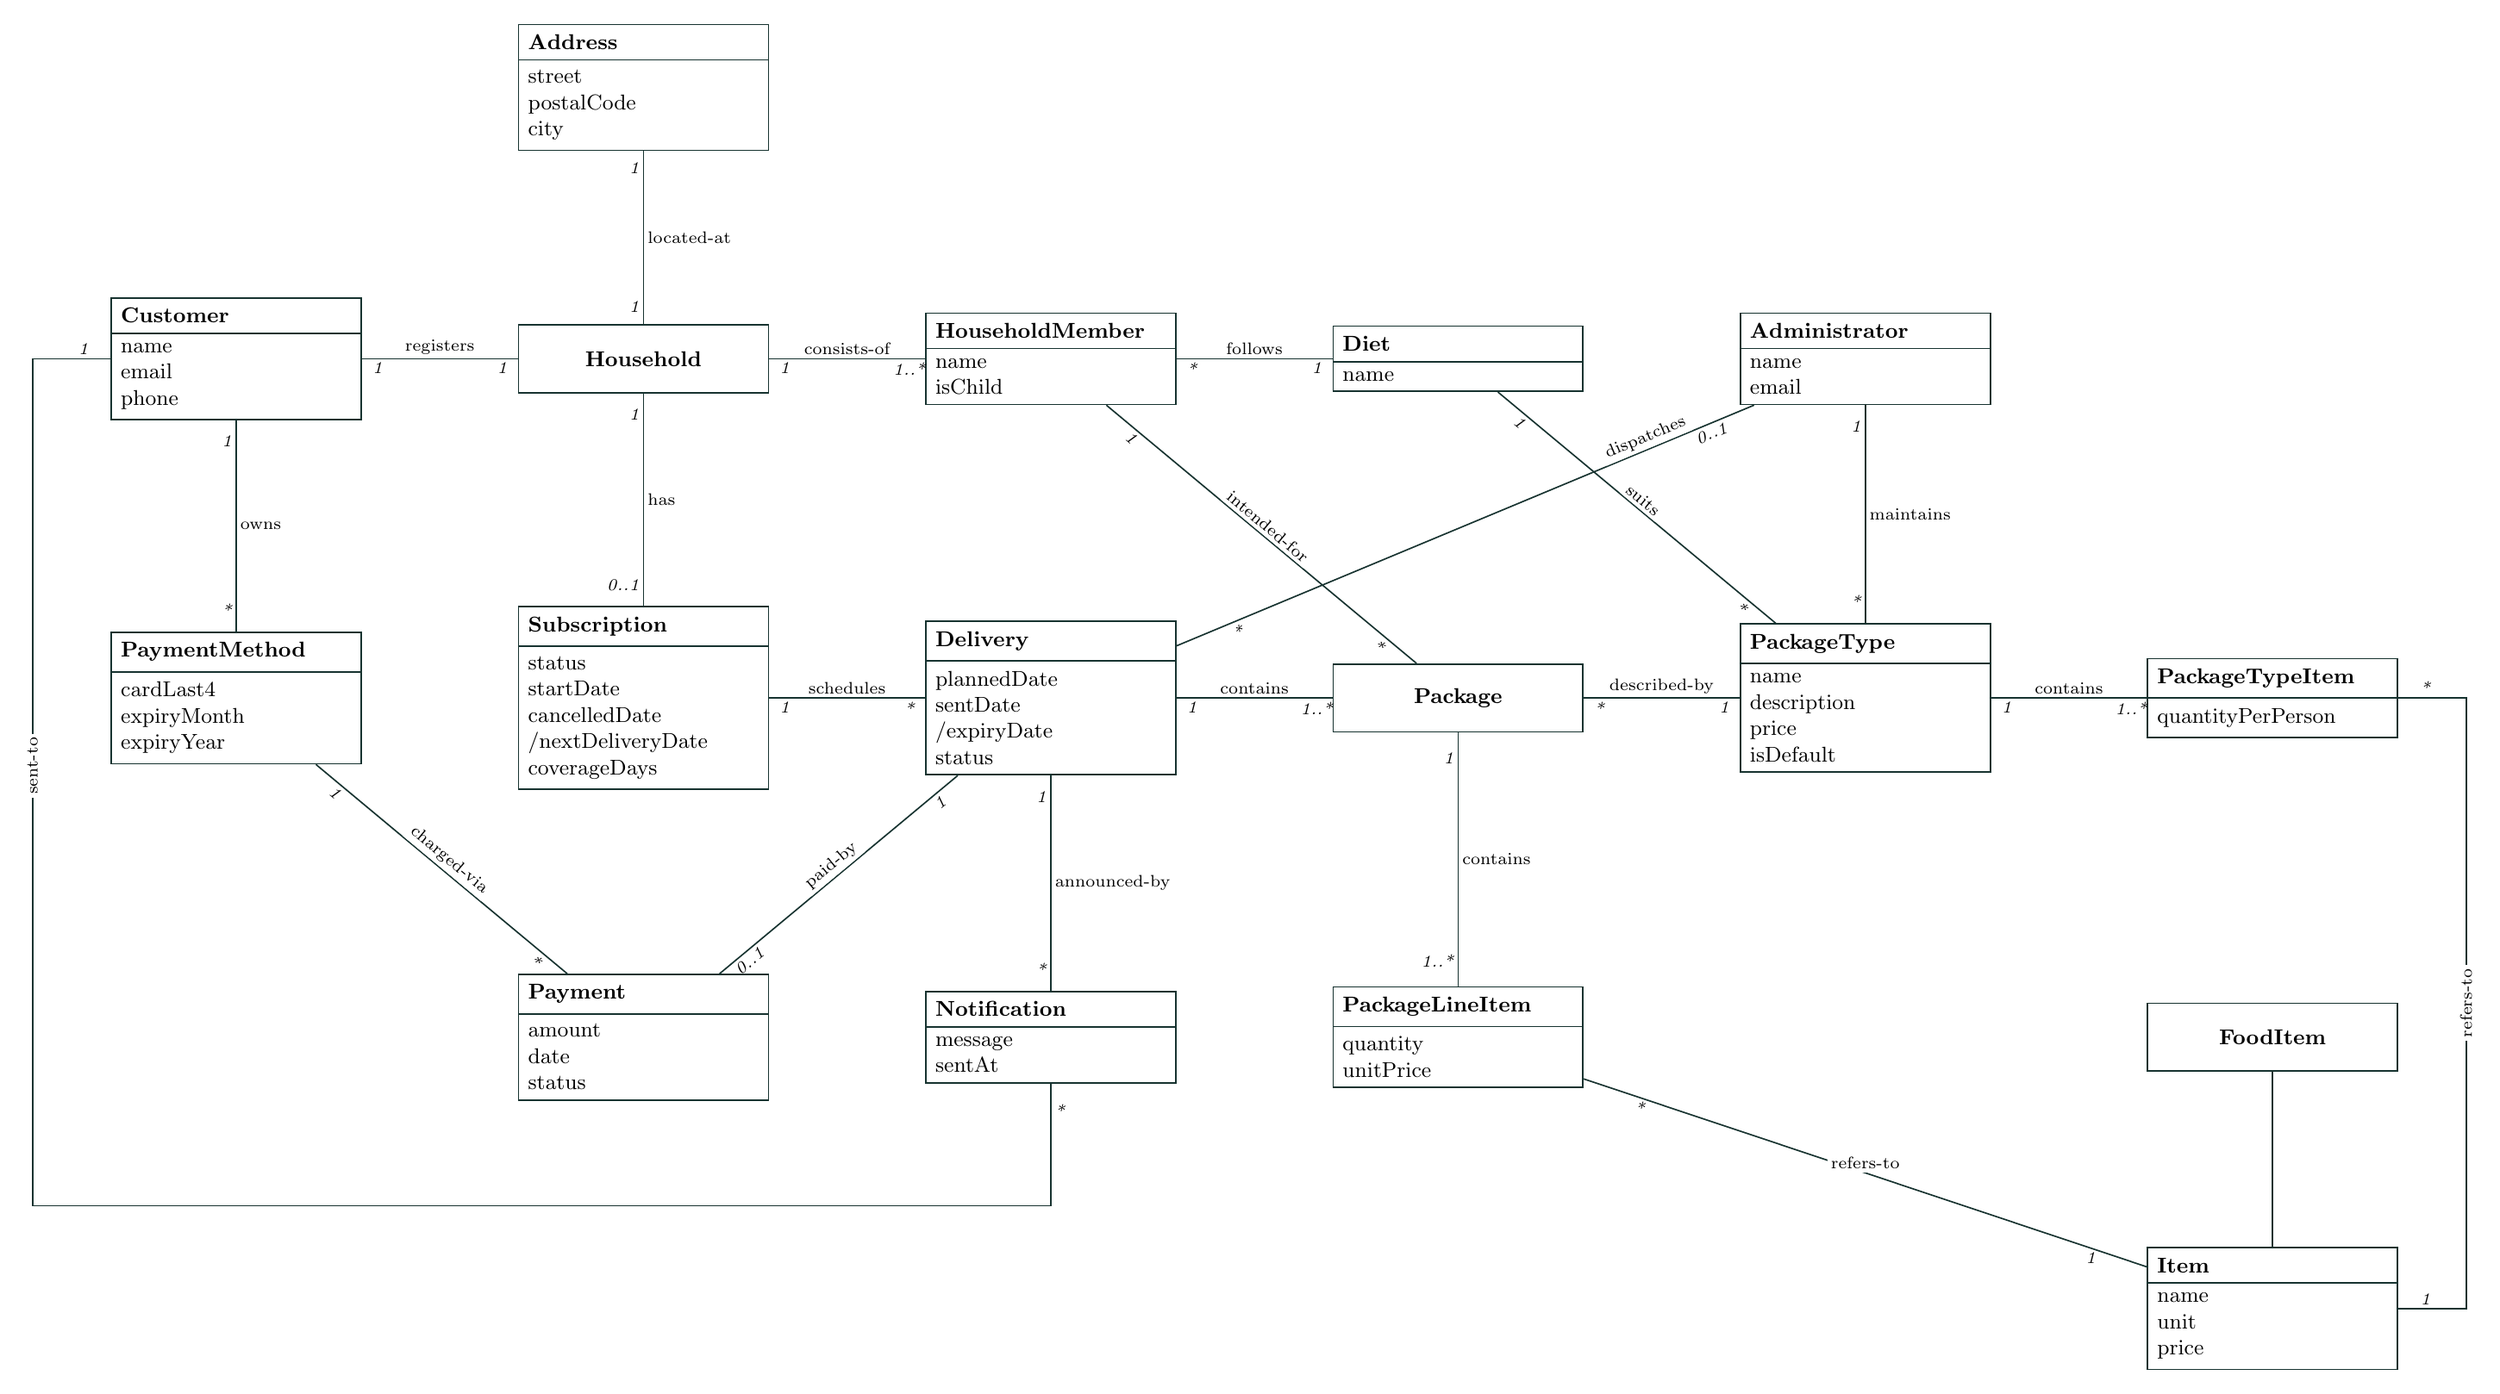
\begin{tikzpicture}[x=1mm,y=1mm]

% ----- raekke 0 (over Household) -----
\cls{address}{60,40}{Address}{street\\postalCode\\city}

% ----- raekke 1 -----
\cls{customer}{0,0}{Customer}{name\\email\\phone}
\node[clsn] (household) at (60,0) {Household};
\cls{member}{120,0}{HouseholdMember}{name\\isChild}
\cls{diet}{180,0}{Diet}{name}
\cls{admin}{240,0}{Administrator}{name\\email}

% ----- raekke 2 -----
\cls{paymentmethod}{0,-50}{PaymentMethod}{cardLast4\\expiryMonth\\expiryYear}
\cls{subscription}{60,-50}{Subscription}{status\\startDate\\cancelledDate\\/nextDeliveryDate\\coverageDays}
\cls{delivery}{120,-50}{Delivery}{plannedDate\\sentDate\\/expiryDate\\status}
\node[clsn] (package) at (180,-50) {Package};
\cls{packagetype}{240,-50}{PackageType}{name\\description\\price\\isDefault}
\cls{packagetypeitem}{300,-50}{PackageTypeItem}{quantityPerPerson}

% ----- raekke 3 -----
\cls{payment}{60,-100}{Payment}{amount\\date\\status}
\cls{notification}{120,-100}{Notification}{message\\sentAt}
\cls{packagelineitem}{180,-100}{PackageLineItem}{quantity\\unitPrice}
\node[clsn] (fooditem) at (300,-100) {FoodItem};

% ----- raekke 4 -----
\cls{item}{300,-140}{Item}{name\\unit\\price}

% ----- associationer (navn i midten, multiplicitet ved hver ende) -----
% Hjaelper: \assoc{fra}{til}{navn}{mult ved fra}{mult ved til}{navn-side}{mult-side}
% Navn og multipliciteter saettes paa hver sin side af stregen, saa de ikke kolliderer.
\newcommand{\assoc}[7]{%
  \draw[assoc] (#1) -- node[lbl,#6]{#3}
    node[mult,pos=.1,#7]{#4} node[mult,pos=.9,#7]{#5} (#2);}

% Kunde og husstand
\assoc{customer}{household}{registers}{1}{1}{above}{below}
\assoc{customer}{paymentmethod}{owns}{1}{*}{right}{left}
\assoc{household}{address}{located-at}{1}{1}{right}{left}
\assoc{household}{member}{consists-of}{1}{1..*}{above}{below}
\assoc{member}{diet}{follows}{*}{1}{above}{below}
\assoc{household}{subscription}{has}{1}{0..1}{right}{left}

% Abonnement og levering
\assoc{subscription}{delivery}{schedules}{1}{*}{above}{below}
\assoc{delivery}{package}{contains}{1}{1..*}{above}{below}
\assoc{delivery}{payment}{paid-by}{1}{0..1}{sloped,above}{sloped,below}
\assoc{payment}{paymentmethod}{charged-via}{*}{1}{sloped,above}{sloped,below}
\assoc{delivery}{notification}{announced-by}{1}{*}{right}{left}
% Notification -> Customer: knaekket streg under raekke 3 og op langs venstre kant
\draw[assoc] (notification.south) -- ++(0,-18) -| (-30,0) -- (customer.west);
\node[mult,right] at ($(notification.south)+(0,-4)$) {*};
\node[mult,above] at ($(customer.west)+(-4,0)$) {1};
\node[lbl,rotate=90] at (-30,-60) {sent-to};

% Administrator
% dispatches: label taet paa Administrator, saa den ikke rammer krydset med intended-for
\draw[assoc] (admin) -- node[lbl,sloped,above,pos=.18]{dispatches}
  node[mult,pos=.08,sloped,below]{0..1} node[mult,pos=.9,sloped,below]{*} (delivery);
\assoc{admin}{packagetype}{maintains}{1}{*}{right}{left}

% Pakke, pakketype og varer
\assoc{package}{member}{intended-for}{*}{1}{sloped,above}{sloped,below}
\assoc{package}{packagetype}{described-by}{*}{1}{above}{below}
\assoc{packagetype}{diet}{suits}{*}{1}{sloped,above}{sloped,below}
\assoc{packagetype}{packagetypeitem}{contains}{1}{1..*}{above}{below}
% PackageTypeItem -> Item: knaekket streg uden om FoodItem
\draw[assoc] (packagetypeitem.east) -- ++(10,0) |- (item.east);
\node[mult,above] at ($(packagetypeitem.east)+(4,0)$) {*};
\node[mult,above] at ($(item.east)+(4,0)$) {1};
\node[lbl,rotate=90] at ($(packagetypeitem.east)+(10,-45)$) {refers-to};
\assoc{package}{packagelineitem}{contains}{1}{1..*}{right}{left}
\assoc{packagelineitem}{item}{refers-to}{*}{1}{above}{below}

% FoodItem er en slags Item (ingen arv-notation i domaenemodellen)
\draw[assoc] (fooditem) -- (item);

\end{tikzpicture}
\end{document}
